
% Lab 3 for ENGR 1120 030 031 - Tristan Hill - Fall 2016 - Fall 2017 - Spring 2020
% 
% Introduction to MATLAB 
%
% Scalars and 1-D Matrices (vectors)
 

% Document settings
\documentclass[11pt]{article}
\usepackage[margin=1in]{geometry}
\usepackage[pdftex]{graphicx}
\usepackage{multirow}
\usepackage{setspace}
\usepackage{hyperref}
\usepackage{color,soul}
\usepackage{fancyvrb}
\usepackage{framed}
\usepackage{wasysym}
\usepackage{multicol}

\pagestyle{plain}
\setlength\parindent{0pt}
\hypersetup{
    bookmarks=true,         % show bookmarks bar?
    unicode=false,          % non-Latin characters in Acrobat’s bookmarks
    pdftoolbar=true,        % show Acrobat’s toolbar?
    pdfmenubar=true,        % show Acrobat’s menu?
    pdffitwindow=false,     % window fit to page when opened
    pdfstartview={FitH},    % fits the width of the page to the window
    pdftitle={My title},    % title
    pdfauthor={Author},     % author
    pdfsubject={Subject},   % subject of the document
    pdfcreator={Creator},   % creator of the document
    pdfproducer={Producer}, % producer of the document
    pdfkeywords={keyword1} {key2} {key3}, % list of keywords
    pdfnewwindow=true,      % links in new window
    colorlinks=true,       % false: boxed links; true: colored links
    linkcolor=red,          % color of internal links (change box color with linkbordercolor)
    citecolor=green,        % color of links to bibliography
    filecolor=magenta,      % color of file links
    urlcolor=blue           % color of external links
}

% assignment number 
\newcommand{\NUM}{4} 
\newcommand{\VSpaceSize}{2mm} 
\newcommand{\HSpaceSize}{2mm} 

\definecolor{mygray}{rgb}{.6, .6, .6}

\setulcolor{red} 
\setstcolor{green} 
\sethlcolor{mygray} 

\begin{document}

	\textbf{\LARGE ENGR 1120 - 800 - Spring 2020} \\\\
	\textbf{\LARGE Lab \NUM \hspace{2mm}- Scalars, 1-D Matrices, and Plotting} 
		
	\begin{description}
	\vspace{5mm}
		\item [\textbf{ \Large Overview}] \textbf{ \Large :}\\
			Previously you used {\it Scalar} variables, where each variable stored only a single value. As the complexity of the problems we attempt to solve increases it becomes useful to store multiple values under the same variable name. In MATLAB this is called a {\it matrix}, and {\bf MAT}LAB was specifically designed to work with {\it matrices}.

        \begin{description}

            \item \textbf {Initialize} : You can set several or all, of the values in a matrix on a single line. This is optional. Notice the elements are separated by commas.
                \begin{verbatim}
                clear variables
                my_numbers=[5,10,15,20,25];
                \end{verbatim}
            \item \textbf {Assign} : You often set each value in a matrix individually. The assignment operator works just as it does with scalars.			
                \begin{verbatim}
                clear all
                my_numbers(1)=5;
                my_numbers(2)=10;
                my_numbers(3)=15;
                my_numbers(4)=20;		
                \end{verbatim}
            
            You do not have to set them in order. The final order of the values is dependent on the indices you used during assignment.
                \begin{verbatim}
                clear all
                my_numbers(3)=15;
                my_numbers(1)=5;
                my_numbers(2)=10;
                my_numbers(4)=20;			
                \end{verbatim}

            \item \textbf {Access} : You often need to get a value previously stored in an element of a matrix. To begin, we will only access 1 element of the matrix at a time. 
           
                \begin{verbatim}
                x=my_numbers(3);
                y=x-my_numbers(4);
                z=y-my_numbers(1);
                \end{verbatim}	

	\item \textbf {View} : There are several ways to look at the data in you matrix. You can see your whole matrix by simply typing the name in the command window. You can also see a graphical version of you matrix with the {\it plot()} function. 

                \begin{verbatim}
                plot(my_numbers)
                plot(my_numbers,your_numbers)
                \end{verbatim}	
    
        \end{description}		 
\newpage	
        \item [\textbf{ \Large Assignment}] \textbf{ \Large :}\\

        \begin{enumerate}

	\item Find the {\it lab\NUM\textunderscore data.txt} file on ilearn. Download this file or open it in the browser. You should see six columns separated by commas. For this assignment we will be using the fourth and fifth columns. 
	
	\item Initialize two separate arrays of data. One with the {\it East} data and one with the {\it North} data. This data represents the locations of several cities in Tennessee in units of meters. This can be hardcoded.
	
	\item Plot each individual point with a different marker type. Put a star on Cookeville. 

	\item Draw a {\it Black Solid Line} between Cookeville and Carthage. Calculate the distance of this line and print this in this command window.	

	\item Draw a  {\it Red Dashed Line} between Cookeville and Nashville. Calculate the distance of this line and print this in this command window.
	
	\item Draw a {\it Blue Dotted Line} from Livingston to Cookeville to Sparta. Calculate the distance of this line and print this in this command window.

	\item Put a title and axis labels on the figure.  BONUS: Label all city names on the figure using the {\it text} function.
	
        \end{enumerate}
    
    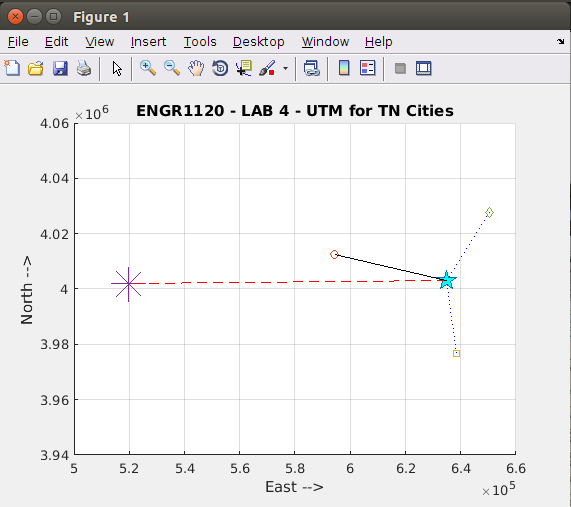
\includegraphics[scale=1]{lab4_fig2.png}
    
    \end{description}
 
\end{document}



